\documentclass[aspectratio=169]{beamer}
\beamertemplatenavigationsymbolsempty

\mode<presentation>
{
        \usetheme{Singapore}
        % \useoutertheme{}
	\setbeamercovered{transparent}
	\setbeamertemplate{footline}[frame number]
}

% \usepackage{flashmovie}
\usepackage[utf8]{inputenc}
\usepackage[T1]{fontenc}
%\usepackage[ngerman]{babel}
\usepackage[english]{babel}
\usepackage{amsmath}
\usepackage[absolute,overlay]{textpos}
\usepackage{svg}

\usebackgroundtemplate{%
\begin{tikzpicture}[remember picture,overlay]
\node[anchor=south west] at (current page.south west) {\includegraphics[height=0.4cm]{by.eps}};
\end{tikzpicture}}

\author[]{Anton Kuzmin}
\institute[]{}
\date[]{@DATE@}

\usepackage{tikz}

\title{GMM-7550 -- Cologne Chip GateMate FPGA Module}
\subtitle{}

\setbeamerfont{table font}{size=\tiny}

\begin{document}

\begin{frame}
  \titlepage
\end{frame}

\section{Intro}

\begin{frame}
  \frametitle{Who am I\dots}
  \begin{itemize}
  \item not a software developer (any more)\\
    \dots but still write code sometimes
  \item developing embedded and real-time systems for almost 30 years
  \item CAMAC, VME, CompactPCI, AdvancedTCA, SoMs
  \item FPGA and SoC-FPGA (Altera/Intel, Microsemi/Microchip)
  \item VHDL
  \end{itemize}
  \vskip.5cm

%  My usual problem with the software is how to make it run on a
%  hardware which is known not to be working yet and how to bring-up
%  and test this hardware. With a soft-core CPU it is getting even
%  worse.

\end{frame}


%\frame{\tableofcontents[subsectionstyle=show]}
\frame{\tableofcontents}

\section{Motivation and Current State}

\begin{frame}
  \frametitle{Why GateMate FPGA}

  %% \vspace{-1.5cm}
  %% \begin{flushright}
  %%   \includegraphics[height=1.5cm]{gatemate-chip.png}
  %% \end{flushright}

  \begin{itemize}
    \item a new kid on the block
    \item FOSS commitment (Yosys for synthesis right now, nextpnr
    in a roadmap)
    \item documented (and partially open) bitstream format
    \item possibility to change configuration at run-time from inside
  \end{itemize}
\end{frame}

\begin{frame}
  \frametitle{Why to design a Module}

  \begin{itemize}
    \item an Evaluation Kit have not been available back in mid 2020
    \item physically smaller
    \item flexibility for experiments (e.g. to interconnect several FPGAs)
    \item best way to get familiar with a new chip
    \item fun and easy exercise with KiCAD (at least it seemed so at the beginning)
  \end{itemize}
\end{frame}

\begin{frame}
  \frametitle{Current Status}
  \begin{itemize}
    \item three boards are designed and manufactured
    \item all the boards are fully functional (from the first versions and
    just a few minor problems)
    \item schematic symbol and PCB footprint for GateMate FPGA are accepted
    into KiCAD libraries
    \item control application is functional enought to debug, test,
    and configure the module
    \item several VHDL examples are running
    \item support for the module is added to the FuseSoC and LiteX
    (work in progress, not upstreamed yet)
    \item \dots it took roughly 5 times longer than initially estimated
  \end{itemize}
\end{frame}

\section{Technical Details}

\subsection{Cologne Chip GateMate FPGA}

\subsection{GMM-7550 Module}

\begin{frame}
  \frametitle{Key Features}
\end{frame}

\begin{frame}
  \frametitle{Power}
\end{frame}

\begin{frame}
  \frametitle{Clock}
\end{frame}

\begin{frame}
  \frametitle{Configuration}
\end{frame}

\subsection{Additional Modules}

\begin{frame}
  \frametitle{Raspberry-Pi 40-pin GPIO HAT Adapter}
\end{frame}

\begin{frame}
  \frametitle{Memory Extension Module}
\end{frame}

\subsection{Software and RTL Code Examples}

\begin{frame}
  \frametitle{Control Application}
\end{frame}

\begin{frame}
  \frametitle{VHDL Examples}
\end{frame}

\begin{frame}
  \frametitle{Third-party Frameworks}
  \begin{itemize}
    \item FuseSoC
    \item LiteX
  \end{itemize}
\end{frame}

\section{What's next}

\section{Contact info}
\begin{frame}

  \begin{minipage}{7cm}
    \vskip.5cm
    \huge{Thank you!}
    \vskip1cm
    \small{Anton Kuzmin}\\
    \small{\texttt{ak-fau+orconf@no-problem.cc}}\\
    \small{\texttt{https://github.com/ak-fau/}}
    \vskip.5cm
    \Huge{Questions?..}
  \end{minipage}

  \vspace{-5cm}
  \begin{flushright}
    \includegraphics[height=5cm]{github-vcard.png}\\
  \end{flushright}

\end{frame}


\end{document}
